%========================
% Document class and theme
%========================
\documentclass[8pt]{beamer}
\usetheme[progressbar=frametitle]{metropolis}
\setbeamersize{text margin left=10mm, text margin right=10mm}
\usepackage{appendixnumberbeamer} % appendix slide numbering
\setbeamertemplate{theorems}[numbered]

%========================
% Core packages
%========================
\usepackage{amsmath, amsfonts, amssymb, amsthm} % math + theorems
\usepackage{booktabs}        % professional tables
\usepackage{hyperref}        % hyperlinks
\usepackage{xcolor}          % colors
\usepackage{xspace}          % spacing for custom commands

%========================
% Algorithms
%========================
\usepackage{algorithm}
\usepackage{algpseudocode}

%========================
% Plots and TikZ
%========================
\usepackage{pgfplots}
\usepgfplotslibrary{dateplot}
\usepackage{tikz}
\usetikzlibrary{positioning}

%========================
% Listings (code)
%========================
\usepackage{listings}
\lstset{
    basicstyle=\ttfamily\small,
    breaklines=true,
    numbers=left,
    numberstyle=\tiny
}

% R style
\lstdefinelanguage{R}{
  morekeywords={TRUE,FALSE},
  deletekeywords={data,frame,length,as,character},
  otherkeywords={0,1,2,3,4,5,6,7,8,9},
  keywordstyle=\color{blue},
  commentstyle=\color{DarkGreen},
  stringstyle=\color{DarkGreen},
  basicstyle=\ttfamily\small
}

% Python style
\lstdefinelanguage{PythonCustom}{
  language=Python,
  keywordstyle=\color{blue},
  commentstyle=\color{gray},
  stringstyle=\color{red},
  basicstyle=\ttfamily\small
}

%========================
% Custom commands
%========================
\newcommand{\themename}{\textbf{\textsc{metropolis}}\xspace}

%========================
% Custom footline
%========================
\setbeamertemplate{footline}
{%
  \leavevmode%
  \hbox{%
  \begin{beamercolorbox}[wd=.35\paperwidth,ht=2.5ex,dp=1.5ex,center]{author in head/foot}%
    \usebeamerfont{author in head/foot}\insertshortauthor
  \end{beamercolorbox}%
  \begin{beamercolorbox}[wd=.3\paperwidth,ht=2.5ex,dp=1ex,center]{title in head/foot}%
    \usebeamerfont{title in head/foot}\insertshorttitle
  \end{beamercolorbox}%
  \begin{beamercolorbox}[wd=.3\paperwidth,ht=2.5ex,dp=1ex,right]{date in head/foot}%
    \usebeamerfont{date in head/foot}\insertframenumber{} / \inserttotalframenumber
  \end{beamercolorbox}}%
  \vskip0pt%
}

%========================
% Beamer tweaks
%========================
\setbeamertemplate{navigation symbols}{} % remove default navigation symbols


%%%%%%%%%%%%%%%%%%%%%%%%%%%%%%%%%%%%%%%%%%%%%%%%%%%%%%%%%%%%%%%%%%%%
%%%%%%%%%%%%%%%%%%%%%%%%%%%%%%%%%%%%%%%%%%%%%%%%%%%%%%%%%%%%%%%%%%%%
% AQUI SE DEFINEN LAS IMAGENES PARA UTILIZAR DESPUES
%\pgfdeclareimage[interpolate=true, height=7cm,width=16cm]{halton-points}{halton-points}
%\pgfdeclareimage[interpolate=true, height=3cm, width =4cm]
%{serie-petroleo-reducido}{serie-petroleo-reducido}
%\pgfdeclareimage[interpolate=true, height=3cm, width =4cm]{rectangle-triangle}{rectangle-triangle}
%\pgfdeclareimage[interpolate=true, height=3cm, width =4cm]{any-angle}{any-angle}
%\pgfdeclareimage[interpolate=true, height=3cm, width =4cm]{Pythagoras}{Pythagoras}


\title{Chapter 2 - Simulating Statistical Models}
\subtitle{Multivariate Normal Distributions. Hierarchical Models.}
\author{Prof. Alex Alvarez, Ali Raisolsadat}
\institute{School of Mathematical and Computational Sciences \\ University of Prince Edward Island}
\date{} % leave empty or add \today
%\title[Stat 4110]{Stat 4110 Statistical Simulation}
%\subtitle{}
%\author[University of Prince Edward Island]{School of Mathematical and Computational Sciences \\ University of Prince Edward Island}

%========================
% Begin document
%========================
\begin{document}

%-------------------
% Title frame
%-------------------
\maketitle

%-------------------
% Slide 1: Linear Algebra Review
%-------------------
\begin{frame}{Linear Algebra Review}

\begin{definition}[Positive Definite Matrices]
A square matrix is called positive definite if it is symmetric and all its eigenvalues 
$\lambda$ are positive, that is $\lambda > 0$.
\end{definition}

\begin{theorem}
If $A$ is positive definite, then it is invertible and $\det(A) > 0$.
\end{theorem}

\begin{theorem}[Symmetric, Positive Definite Matrix -- SPD]
A symmetric matrix $A$ is positive definite if and only if 
$\mathbf{x}^T A \mathbf{x} > 0$ for every column $\mathbf{x} \neq 0 \in \mathbb{R}^d$.
\end{theorem}

\begin{theorem}
The following conditions are equivalent for a symmetric $n \times n$ matrix $A$: 
\begin{enumerate}
\item $A$ is positive definite.
\item $\det(A) > 0$ and for each principal submatrix $\det({}^{(r)}A)$ for $r = 1, 2, \dots, n$.
\item $A = LU$, where $L$ is unit lower triangular and $U$ is upper triangular with positive entries on the main diagonal.
\end{enumerate}
\end{theorem}

\begin{theorem}
If $A \in \mathbb{R}^{d \times d}$ is SPD, the decomposition $A = LU$, where $L$ is unit lower triangular and $U$ is upper triangular, exists and is unique. 
\end{theorem}
\end{frame}


%-------------------
% Slide 2: Cholesky Decomposition
%-------------------
\begin{frame}{Cholesky Decomposition}
\begin{theorem}[Cholesky Decomposition]
If $A \in \mathbb{R}^{d \times d}$ is SPD, the decomposition $A = LL^{T}$, where $L$ is a lower triangular matrix with strictly positive diagonal elements, exists and is unique. 
\end{theorem}


The expressions for the elements $l_{ij}$ of $L$ can be obtained from
\begin{equation*}
a_{ij} = \sum_{k = 1}^{n} (L)_{ik}(L^{T})_{kj} = \sum_{k=1}^{\min(i,j)}l_{ik}l_{jk}
\end{equation*}
where we have used the matrix element notation $(L)_{ik} = l_{ik}$, which implies $(L^T)_{kj} = l_{jk}$. It suffices this expression for $j \leq i$, i.e., 
\begin{equation*}
a_{ij} = \sum_{k = 1}^{j}l_{ik}l_{jk} = \sum_{k=1}^{j-1}l_{ik}l_{jk} + l_{ij}l_{jj} \quad \text{for} j \leq i
\end{equation*}

\vspace{2mm}

This leads to the following expressions for the matrix elements of $L$:
\begin{equation*}
l_{ij} = \frac{1}{l_{jj}} \biggl(a_{ij} - \sum_{k=1}^{j-1} l_{ik}l_{jk}\biggr) \quad  \text{for $j < i$}
\end{equation*}
\begin{equation*}
l_{ii} = \sqrt{a_{ii} - \sum_{k=1}^{i-1}l_{ik}^{2}}
\end{equation*}
\end{frame}

%-------------------
% Slide 3: Cholesky Decomposition Algorithm
%-------------------
\begin{frame}{Cholesky Decomposition Algorithm}
\begin{algorithm}[H]
\caption{Cholesky Decomposition}\label{alg:cholesky-decomposition}
\begin{algorithmic}[1]
  \State \textbf{Input:} Matrix $A$
  \For{$i=1$ to $n$}
    \For{$j=1$ to $i-1$}
      \State $l_{ij} = \frac{1}{l_{jj}} \biggl(a_{ij} - \sum_{k=1}^{j-1} l_{ik}l_{jk}\biggr)$
    \EndFor
    \State $l_{ii} = \sqrt{a_{ii} - \sum_{k=1}^{i-1}l_{ik}^{2}}$
  \EndFor
  \State \textbf{Output:} Cholesky factor $L$
\end{algorithmic}
\end{algorithm}

The computational work is given by 
$$W = \sum_{i=1}^{n}\sum_{j=1}^{i}(1 M/S + (j-1)M + (j-1)A) \quad \text{flops}$$
where $S$ stands for square root, which is assumed to take the same amount of time as a multiplication or addition, and $M/S$ means multiplication or a square root operation). We can solve this to get
$$W = \frac{n^3}{3}+O(n^2) \quad \text{flops}$$
\end{frame}

%-------------------
% Slide 4: Multivariate Normal Distributions
%-------------------
\begin{frame}{Multivariate Normal Distributions}
\textbf{Multivariate Normal Distributions}

\vspace{3mm}

Let $\mu \in \mathbb{R}^d$ be a vector and $\Sigma \in \mathbb{R}^{d \times d}$ is a symmetric, positive definite matrix. Then a random vector $X\in \mathbb{R}^d$ is normally distributed with mean $\mu$ and covariance matrix $\Sigma$, if the distribution of $X$ has density $f: \mathbb{R}^d \rightarrow \mathbb{R}$ given by:
\begin{equation*}
f(x)=\frac{1}{(2\pi)^{d/2} |\det \Sigma| ^{1/2}}
\exp\left(-\frac{1}{2}(x-\mu)^T\Sigma^{-1}(x-\mu) \right)
\end{equation*}
for all $x \in \mathbb{R}^d$.
\end{frame}

%-------------------
% Slide 5: Multivariate Normal Distributions
%-------------------
\begin{frame}{Multivariate Normal Distributions}
In the one dimensional case we know that if $Z \sim N(0,1)$ and $\mu, \sigma \in \mathbb{R}$, then the random variable $Y=\sigma Z+\mu$ is also normally distributed, moreover $Y \sim N(\mu, \sigma^2)$. 
\vspace{2mm}

We have a similar result in the multidimensional case (Lemma 2.2 from the textbook)
\vspace{2mm}

{\bf Lemma:} Let $\mu \in \mathbb{R}^d$ and $A  \in \mathbb{R}^{d \times d}$   be invertible. Define $\Sigma=A A^T \in \mathbb{R}^{d \times d}$. Furthermore, let $Z=(Z_1,Z_2, \ldots Z_d)^T$ be a vector of independent, identically distributed random variables with standard normal distribution. Then,$$Y=AZ+\mu \sim N(\mu, \Sigma)$$
on $\mathbb{R}^d$ (show proof on assignment).
\end{frame}

%-------------------
% Slide 6: Simulation from a Multivariate Normal Distribution
%-------------------
\begin{frame}{Simulation from a Multivariate Normal Distribution}
The previous result is the basis for a general algorithm to generate 
multivariate normal random vectors with distribution 
$N(\mu, \Sigma)$.

\vspace{2mm}

\begin{algorithm}[H]
\caption{Simulation from a Multivariate Normal Distribution}\label{alg:mvnormal}
\begin{algorithmic}[1]
  \State \textbf{Input:} mean vector $\mu \in \mathbb{R}^d$, covariance matrix $\Sigma \in \mathbb{R}^{d \times d}$
  \State Find a matrix $A$ such that $A A^T = \Sigma$ \Comment{Cholesky factorization}
  \State Generate $Z = (Z_1, Z_2, \dots, Z_d)^T$ with $Z_i \sim \mathcal{N}(0,1)$ i.i.d.
  \State Compute $X = AZ + \mu$
  \State \textbf{Output:} $X \sim N(\mu, \Sigma)$
\end{algorithmic}
\end{algorithm}
\end{frame}

%-------------------
% Slide 7: Multivariate Normal Distributions
%-------------------
\begin{frame}{Multivariate Normal Distributions}
\textbf{Remarks}:
\begin{itemize}
	\item One key step is to find a matrix $A$ such that $AA^T=\Sigma$.
Possibly the most straightforward way to do this is by using the Cholesky decomposition of (positive definite) matrix $\Sigma$.
	\item In {\bf R}, the  matrix $A$ can be obtained by applying the function \textbf{chol} to matrix $\Sigma$ and transposing the resulting matrix. 
	\item In \textbf{Python} can be performed efficiently using the \textbf{numpy.linalg.cholesky} function or the \textbf{scipy.linalg.cholesky} function. 
	\item While the components of $Z$ are independent, the components of $X$ are dependent random variables in general.
	\item Most standard statistical software have built-in functions to generate normal vectors of arbitrary dimension. What we are learning to do here is generating these vectors from scratch.
\end{itemize}
\end{frame}

%-------------------
% Slide 8: Multivariate Normal Distributions (Chelosky Example)
%-------------------
\begin{frame}{Multivariate Normal Distributions -- Example}
\textbf{Example}: Generate a sample of 100 random vectors in $\mathbb{R}^2$ that follow the normal distribution with mean 
$\mu=\left[\begin{array}{l} 4 \\ 2\end{array}\right]$ and covariance matrix $\Sigma=\left[\begin{array}{ll} 1 & 2\\ 2 & 9\end{array}\right]$

\vspace{2mm}

\textbf{Matrix $A$}:
\begin{equation*}
\Sigma = AA^T = \left[\begin{array}{ll} l_{11} & 0\\ l_{21} & l_{22}\end{array}\right]\left[\begin{array}{ll} l_{11} & l_{21}\\ 0 & l_{22}\end{array}\right]
\end{equation*}
\begin{equation*}
l_{11} = \sqrt{a_{11}}, \quad l_{21} = \frac{1}{l_{11}} a_{21}, \quad l_{22} = \sqrt{a_{22}-l_{21}^{2}}
\end{equation*}
\begin{equation*}
l_{11} = \sqrt{1}, \quad l_{21} = \frac{1}{1}2 = 2, \quad l_{22} = \sqrt{9 - 2^2} = \sqrt{5}
\end{equation*}
So
\begin{equation*}
\Sigma = AA^T = \left[\begin{array}{ll} 1 & 0\\ 2 & \sqrt{5} \end{array}\right]\left[\begin{array}{ll} 1 & 2\\ 0 & \sqrt{5}\end{array}\right] = \left[\begin{array}{ll} 1 & 2\\ 2 & 9\end{array}\right]
\end{equation*}
\end{frame}

%-------------------
% Slide 9: Multivariate Normal Distributions (Chelosky Example) Plot
%-------------------
\begin{frame}{Multivariate Normal Distributions -- Example}
\begin{center}
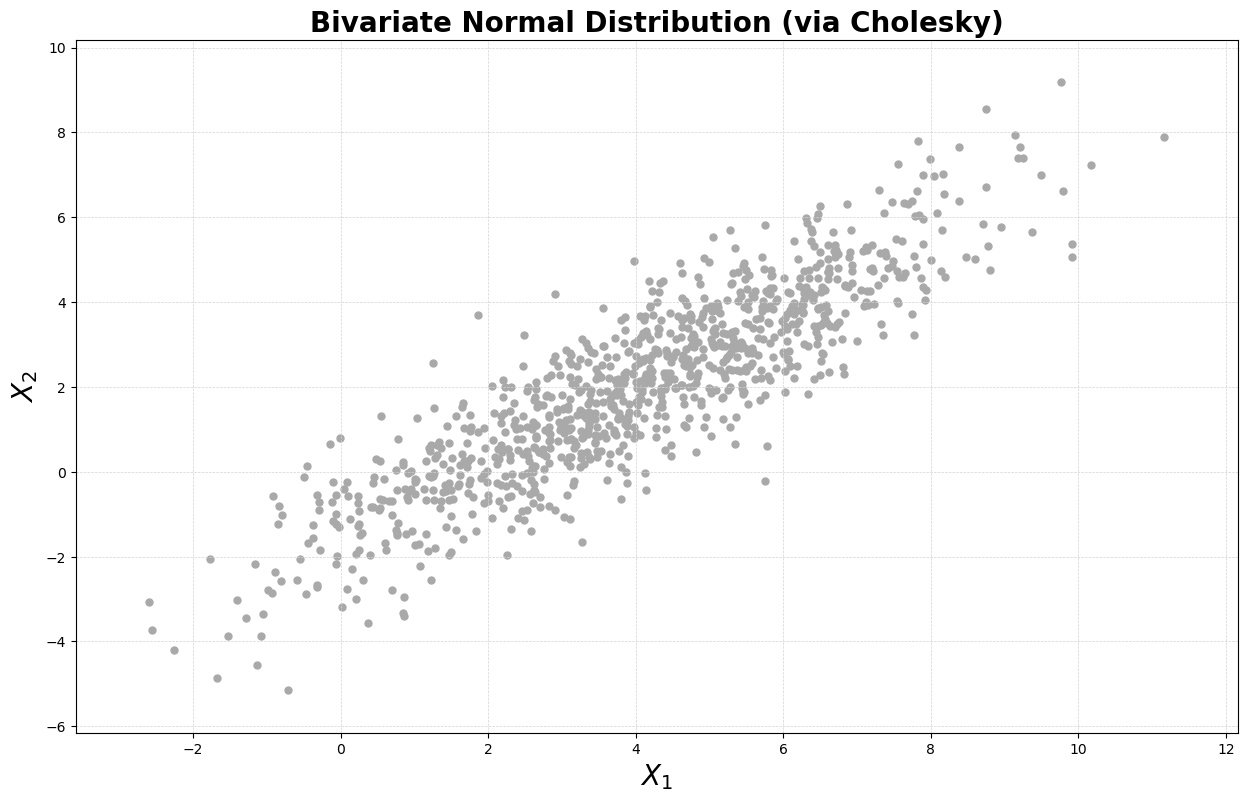
\includegraphics[width=\textwidth]{chapter2-part1-plot1.png}
\end{center}
\end{frame}


%-------------------
% Slide 10: Hierarchical models
%-------------------
\begin{frame}{Hierarchical models}
Some statistical models have a hierarchical structure in the sense that not all random variables are defined simultaneously. Instead there exist several levels of randomness and the random variables in some levels depend on the variables defined in earlier levels. Some examples of these hierarchical models that are covered in our textbook are:

\vspace{2mm}

\begin{itemize}
	\item \textbf{Bayesian models} in which the parameters that defined the distribution of the data are not fixed but themselves are random variables.
	\item \textbf{Mixture models} that combine sub-populations that follow different distributions
	\item \textbf{Markov Chains} in which the distribution of the value at time $t$ depends on the value of the Markov Chain at time $t-1$ (we will cover this topic separately).
\end{itemize}
\end{frame}

%-------------------
% Slide 11: Bayesian Models
%-------------------
\begin{frame}{Bayesian Models}
Simulation of data that is distributed according to a Bayesian model is done in steps, by following the structure of the model. 

\vspace{3mm}

\textbf{Example 2.5 from textbook}: Consider a Bayesian model where the data are described as i.i.d. sample $X_1, X_2, \ldots X_n \sim N(\mu, \sigma^2)$ where the mean $\mu$ and the variance $\sigma^2$ are themselves assumed to be random with distribution $\sigma^2 \sim \text{Exp}(\lambda)$ and $\mu \sim N(\mu_0, \alpha \sigma^2)$.

In a model like this the distribution of $\mu$ depends on $\sigma^2$ so the model has the following dependence structure:
\begin{equation*}
\sigma^2 \;\;\;\; \longrightarrow \;\;\;\; \mu \;\;\;\; \longrightarrow \;\;\;\; X_1, X_2, \ldots X_n
\end{equation*}

We describe the model in terms of conditional probabilities:
\begin{equation*}
\begin{aligned}
X_i \mid \mu, \sigma^2 &\sim N(\mu, \sigma^2), \quad i=1,\dots,n, \\
\mu \mid \sigma^2 &\sim N(\mu_0, \alpha\sigma^2), \\
\sigma^2 &\sim \text{Exp}(\lambda).
\end{aligned}
\end{equation*}
\end{frame}

%-------------------
% Slide 12: Bayesian Model Simulation Algorithm
%-------------------
\begin{frame}{Bayesian Model Simulation Algorithm}
\begin{algorithm}[H]
\caption{Generate data from the Bayesian model}\label{alg:bayesian-model}
\begin{algorithmic}[1]
  \State \textbf{Input:} parameters $\lambda, \mu_0, \alpha$, and sample size $n$
  \State Generate $\sigma^2 \sim \text{Exp}(\lambda)$
  \State Generate $\mu \sim N(\mu_0, \alpha\sigma^2)$
  \For{$i=1$ to $n$}
    \State Generate $X_i \sim N(\mu, \sigma^2)$
  \EndFor
  \State \textbf{Output:} $X = (X_1, X_2, \dots, X_n)$
\end{algorithmic}
\end{algorithm}

\vspace{2mm}

\textbf{Remark:} The parameters $\lambda, \mu_0, \alpha$ are fixed and assumed known.

\vspace{2mm}

\textbf{Example}: Generate a sample of 1000 random numbers following this other type of Bayesian hierarchical model (not present in the textbook) with $\lambda=1$, $\mu_0=5$, $\alpha=2$.
\end{frame}

%-------------------
% Slide 13: Bayesian Model Simulation Plot
%-------------------
\begin{frame}[fragile]{Bayesian Model Simulation Histogram - Method 1}
\begin{center}
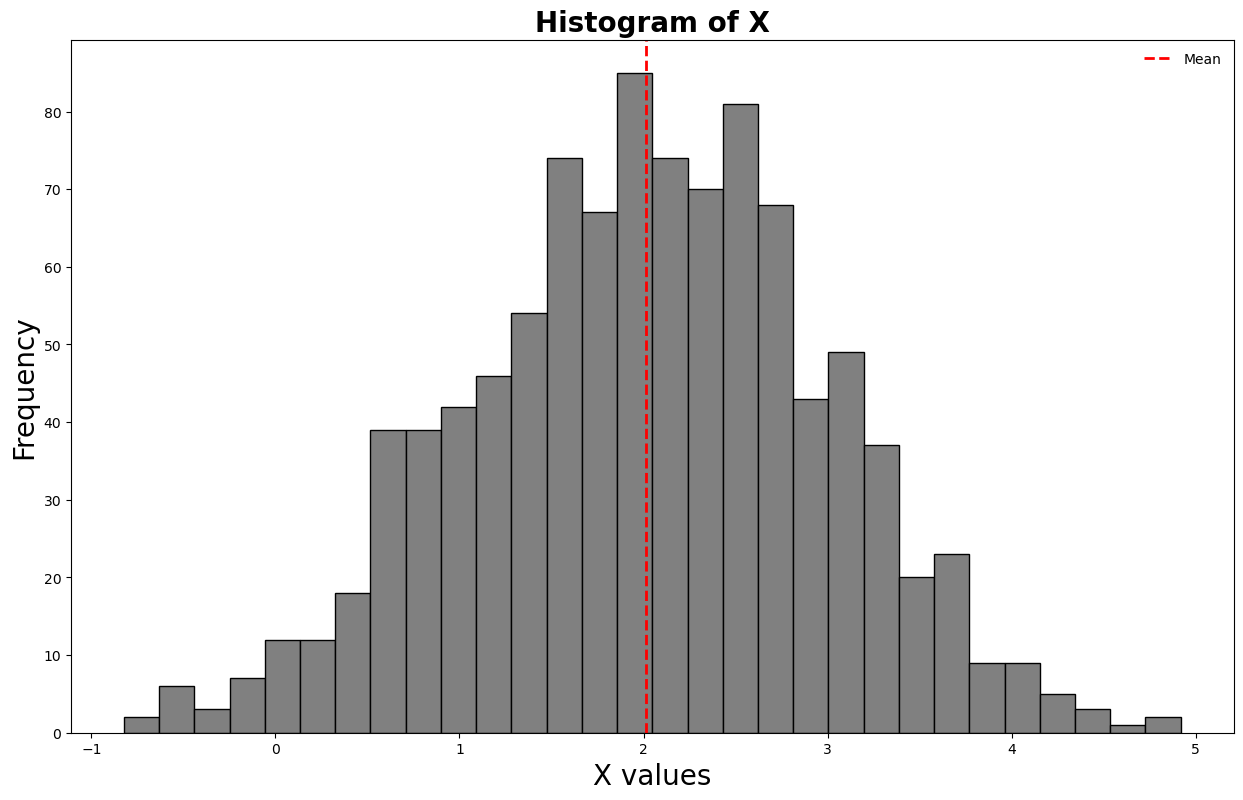
\includegraphics[width=\textwidth]{chapter2-part1-plot2.png}
\end{center}
\end{frame}

%-------------------
% Slide 14: Bayesian Model Simulation Algorithm
%-------------------
\begin{frame}{Bayesian Model Simulation Algorithm}
\begin{algorithm}[H]
\caption{Simulation from a Bayesian Model}\label{alg:bayesian-sim}
\begin{algorithmic}[1]
  \For{$i = 1$ to $n$}
    \State Generate $\sigma^2 \sim \text{Exp}(\lambda)$
    \State Generate $\mu \sim N(\mu_0, \alpha \sigma^2)$
    \State Generate $X_i \sim N(\mu, \sigma^2)$
  \EndFor
  \State \textbf{Output:} $X = (X_1, X_2, \dots, X_n)$
\end{algorithmic}
\end{algorithm}

\vspace{2mm}

\textbf{Remark:} Depending on the type of sample that we want to generate, 
different versions of the algorithm can be implemented.

\vspace{2mm}

\textbf{Example}: Generate a sample of 1000 random numbers following this other type of Bayesian hierarchical model (not present in the textbook) with $\lambda=1$, $\mu_0=5$, $\alpha=2$.
\end{frame}

%-------------------
% Slide 15: Bayesian Model Simulation Plot
%-------------------
\begin{frame}[fragile]{Bayesian Model Simulation Histogram - Method 2}
\begin{center}
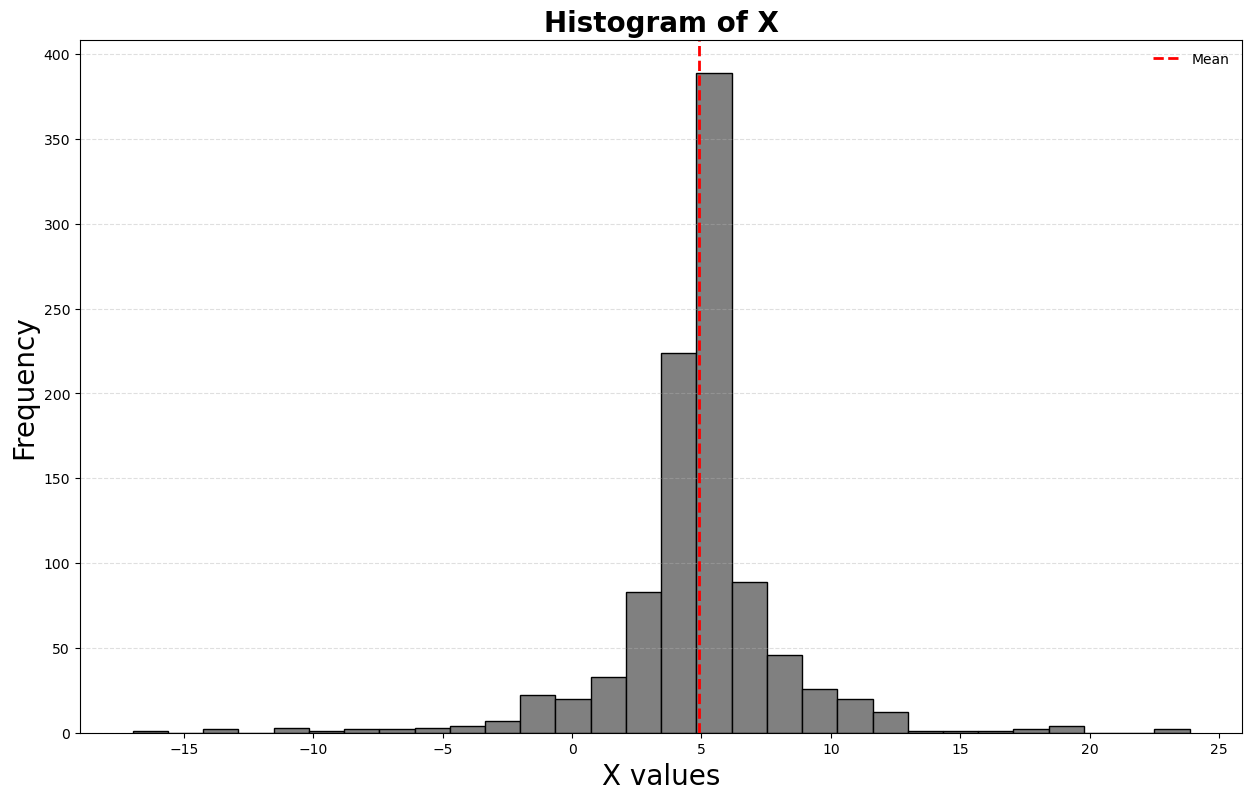
\includegraphics[width=\textwidth]{chapter2-part1-plot3.png}
\end{center}
\end{frame}

%-------------------
% Slide 16: Mixture Models
%-------------------
\begin{frame}{Mixture Models}
\textbf{Mixture Models:}

\vspace{2mm}

Mixture models are typically used to represent the presence of subpopulations within an overall population. 
\vspace{2mm}

Consider probabilities distributions with densities $f_1,f_2, \ldots f_k$ and weights $\omega_1, \omega_2, \ldots \omega_k >  0$ such that 
$\displaystyle{\sum_{i=1}^k \omega_i =1}$, then we can construct a mixture distribution with density

$$f=\sum_{i=1}^k \omega_i f_i$$
\end{frame}

%-------------------
% Slide 17: Generation of Random Numbers from a Mixture Distribution
%-------------------
\begin{frame}{Generation of Random Numbers from a Mixture Distribution}
\begin{algorithm}[H]
\caption{Simulation from a Mixture Distribution}\label{alg:mixture}
\begin{algorithmic}[1]
  \State \textbf{Input:} weights $(\omega_1, \dots, \omega_k)$, component densities $(f_1, \dots, f_k)$
  \State Generate a discrete random variable $Y$ such that 
        $\mathbb{P}(Y=i) = \omega_i$
  \State Generate $X \sim f_Y$
  \State \textbf{Output:} $X$
\end{algorithmic}
\end{algorithm}

\vspace{2mm}

\textbf{Remarks:}  
\begin{itemize}
  \item To generate a sample of size $n$, repeat steps 1–3 $n$ times.  
  \item For large $n$, the weights $\omega_i$ approximate the proportions of observations generated from each component $f_i$.  
\end{itemize}
\end{frame}

%-------------------
% Slide 18: Generation of Random Numbers from a Mixture Distribution
%-------------------
\begin{frame}{Example (Mixture Distribution)}
Generate a sample of 1000 random numbers from the mixture distribution of:\\
Distribution 1: $N(-1,4)$  and \\
Distribution 2: $N(5,1)$  \\
with weights $\omega_1=0.4$ and $\omega_2=0.6$. \\

\vspace{2mm}

\alert{Steps for Code}
\begin{itemize}
	\item \textbf{for} $i=1 \text{ to } 1000$ \textbf{do}:
		\begin{itemize}
			\item Generate $U \sim U[0,1]$
			\item \textbf{If} $U<0.4$ then generate $X[i] \sim N(-1,4)$
			\item \textbf{If} $U>0.4$ then generate $X[i] \sim N(5,1)$
		\end{itemize}
	\item end \textbf{for}
	\item \textbf{Output}: $X=(X[1],X[2],...X[1000])$
\end{itemize}
\end{frame}

%-------------------
% Slide 19: Mixture Distribution vs. Mixture of Random Variables
%-------------------
\begin{frame}[fragile]{Mixture Distribution Example}
\begin{center}
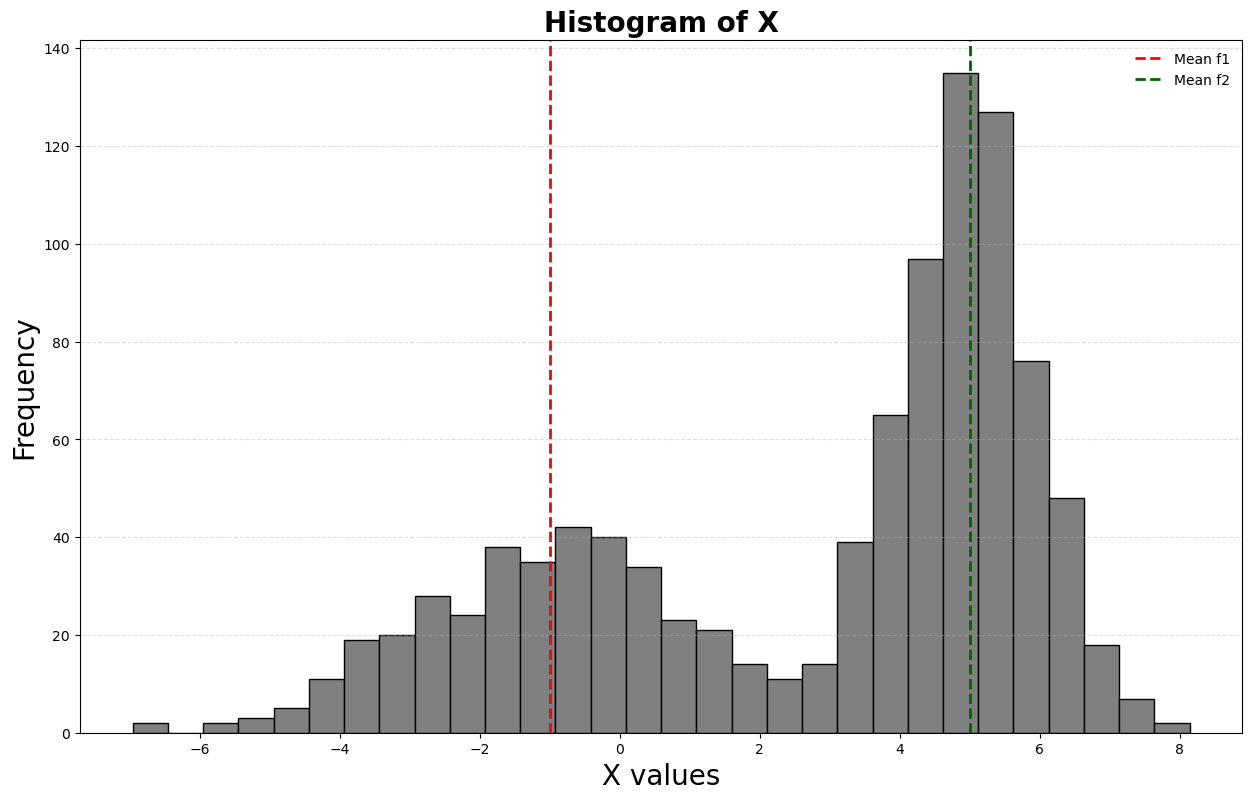
\includegraphics[width=\textwidth]{chapter2-part1-plot4.png}
\end{center}
\end{frame}

%-------------------
% Slide 20: Mixture Distribution vs. Mixture of Random Variables
%-------------------
\begin{frame}[fragile]{Mixture Distribution vs. Mixture of Random Variables}
\textbf{Remark}: The mixture distribution is a weighted sum of distributions. \alert{It is not the distribution of a weighted sum of random variables}

\vspace{3mm}

{\bf Weighted sum of random variables}

Consider the weighted sum $Y=\omega_1 X_1+\omega_2 X_2$ where
$X_1 \sim N(-1,4)$, \\
$X_2 \sim N(5,1)$  \\
and weights $\omega_1=0.4$ and $\omega_2=0.6$.
\end{frame}

%-------------------
% Slide 21: Mixture Distribution vs. Mixture of Random Variables
%-------------------
\begin{frame}[fragile]{Mixture of Random Variables Example}
\begin{center}
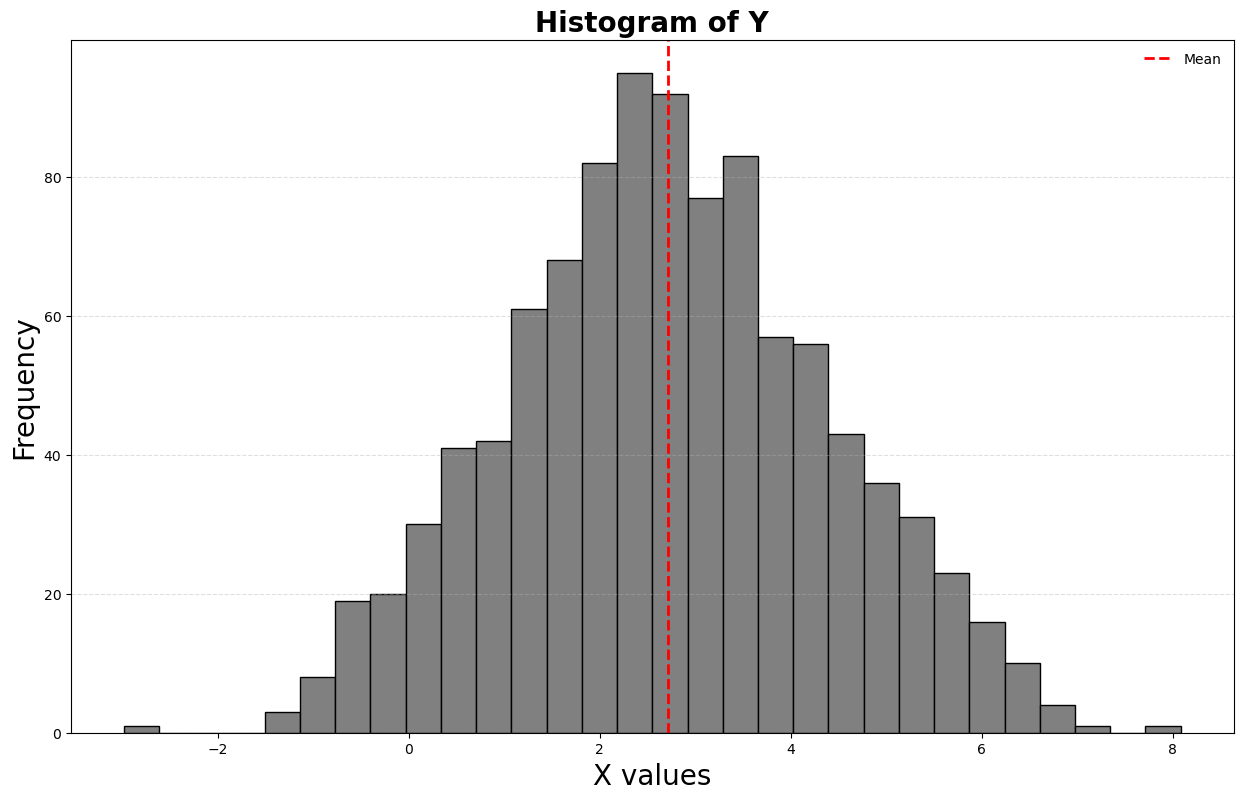
\includegraphics[width=0.95\textwidth]{chapter2-part1-plot5.png}
\end{center}

\vspace{-3mm}

{\bf Remark:} We can clearly see the difference between the histogram of the weighted sum of random variables and the histogram of the mixture distribution.
\end{frame}

%-------------------
% Slide 22: Homework
%-------------------
\begin{frame}{Homework}
\begin{enumerate}
	\item Generate a sample of 1000 random numbers that follow the Bayesian model $X \sim binomial(n+1,p)$ where $p \sim U[0.4, 0.8]$ and $n$ follows the geometric distribution with probability of success $p/2$.
	\item Generate a sample of 1000 random numbers from the mixture distribution of:\\
Distribution 1: Exponential with parameter $\lambda=1$ and \\
Distribution 2: Exponential with parameter $\lambda=1/10$  \\
with weights $\omega_1=0.3$ and $\omega_2=0.7$. \\
\end{enumerate}
\end{frame}


\end{document}